\begin{figure*}
  \vspace{-1.5em}
  \centering
  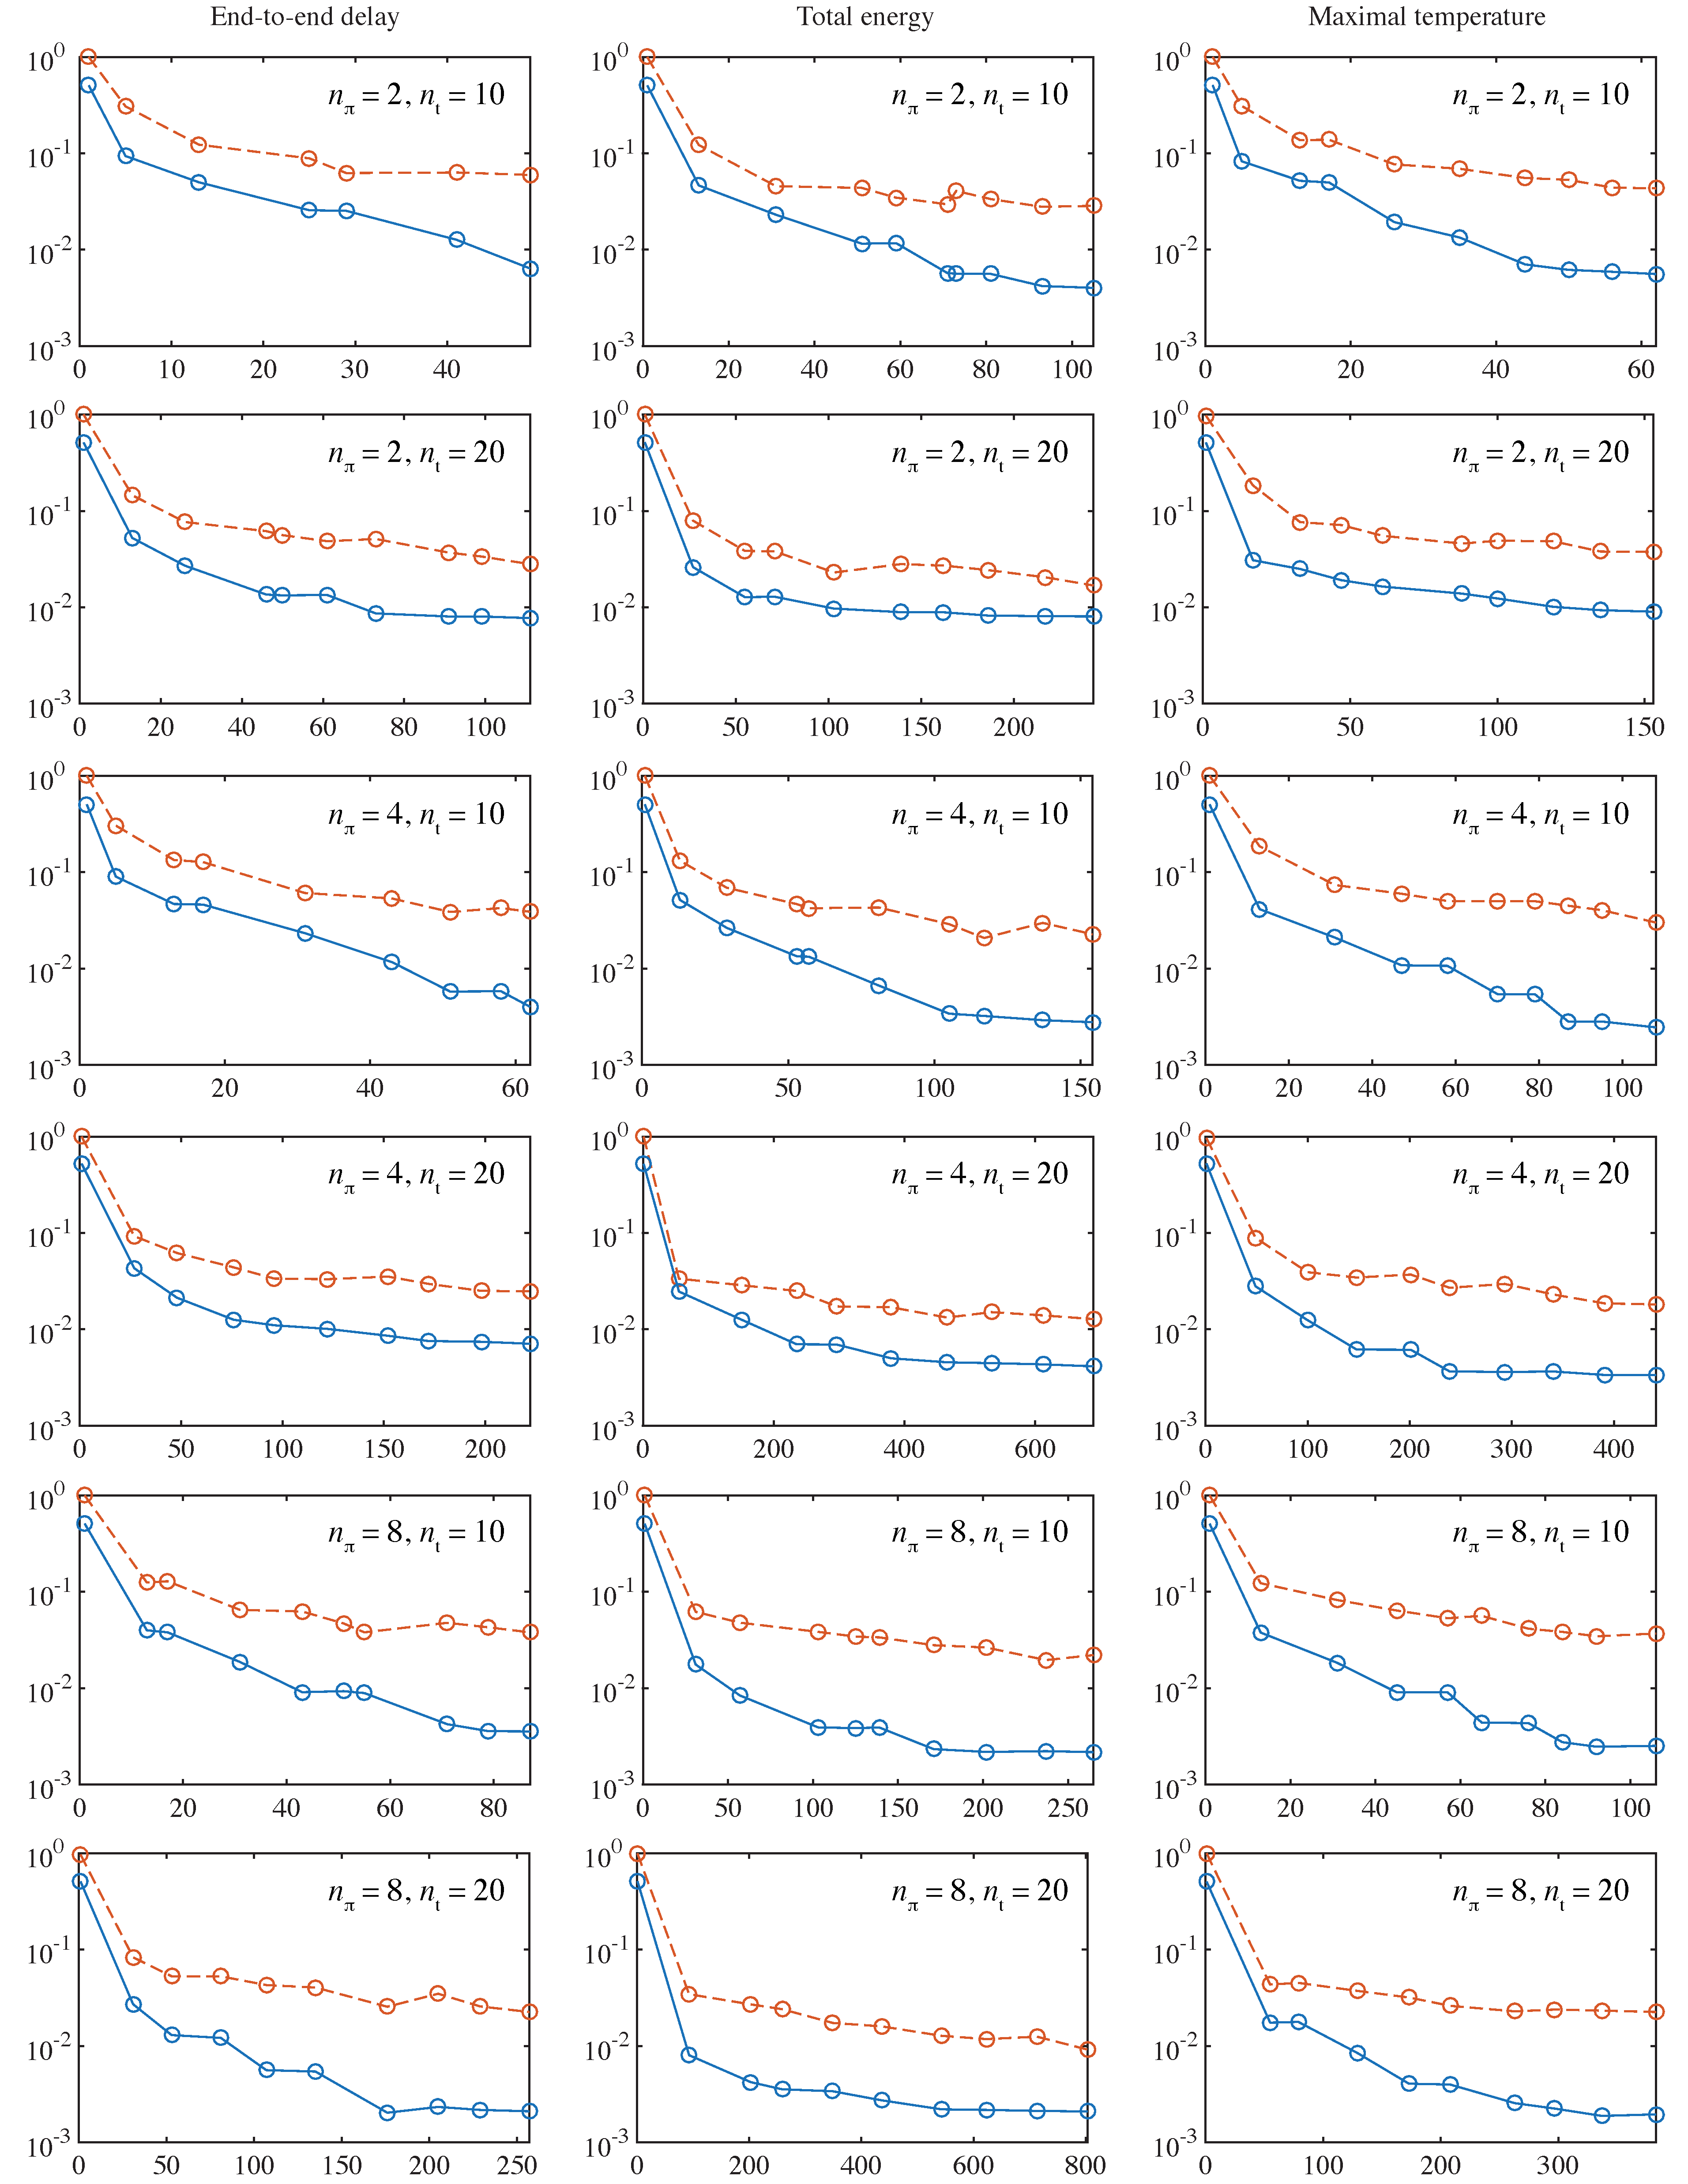
\includegraphics[width=1.0\textwidth]{include/assets/figures/results.pdf}
  \vspace{-1.5em}
  \caption{
    Experimental results. There are considered 3 platform sizes, 2 application
    sizes, and 3 quantities. The columns correspond to the three quantities: the
    end-to-end delay (left), total energy (middle), and maximum temperature
    (right). The three pairs of rows correspond to the three platform sizes: 2
    (top), 4 (middle), and 8 (bottom) processing elements. The rows alternate
    between the two application sizes: 10 (odd) and 20 (even) tasks. The
    horizontal axes show the number of points, and the vertical ones the error
    on a logarithmic scale. The solid lines correspond to our technique, and the
    dashed ones to direct sampling.
  }
  \flab{results}
\end{figure*}
